\documentclass[aspectratio=169]{beamer}
\usetheme{Madrid}
\usecolortheme{default}

% Remove navigation symbols
\setbeamertemplate{navigation symbols}{}

% Customize headline: show current section name on left
\setbeamertemplate{headline}{
    \leavevmode%
    \hbox{%
        \begin{beamercolorbox}[wd=\paperwidth,ht=2.5ex,dp=1ex,left]{section in head/foot}%
            \hspace*{2ex}\usebeamerfont{section in head/foot}\insertsectionhead
        \end{beamercolorbox}}%
    \vskip0pt%
}

% Customize footline: title (2), date (1), page number (1)
\setbeamertemplate{footline}{
    \leavevmode%
    \hbox{%
        \begin{beamercolorbox}[wd=.5\paperwidth,ht=2.25ex,dp=1ex,center]{author in head/foot}%
            \usebeamerfont{author in head/foot}\insertshorttitle
        \end{beamercolorbox}%
        \begin{beamercolorbox}[wd=.25\paperwidth,ht=2.25ex,dp=1ex,center]{title in head/foot}%
            \usebeamerfont{title in head/foot}\insertshortdate
        \end{beamercolorbox}%
        \begin{beamercolorbox}[wd=.25\paperwidth,ht=2.25ex,dp=1ex,right]{date in head/foot}%
            \usebeamerfont{date in head/foot}\insertframenumber{} / \inserttotalframenumber\hspace*{2ex}
        \end{beamercolorbox}}%
    \vskip0pt%
}

\usepackage{graphicx}
\usepackage{amsmath}
\usepackage{tikz}
\usetikzlibrary{patterns,decorations.pathreplacing}
\usepackage{booktabs}

%-----------------------------------------------
% Custom Commands for PowerPoint Integration
%-----------------------------------------------

% Video placeholder command - creates a box indicating where to insert video
\newcommand{\videoplacehold}[2]{%
    \begin{center}
        \begin{tikzpicture}
            \node[draw, thick, minimum width=8cm, minimum height=4cm, fill=gray!10] {%
                \begin{tabular}{c}
                    {\Large \textbf{[VIDEO]}}\\[0.3cm]
                    \textbf{#1}\\[0.2cm]
                    {\small File: \texttt{#2}}
                \end{tabular}
            };
        \end{tikzpicture}
    \end{center}
}

% Presenter section title slide
\newcommand{\presentertitle}[2]{%
    \begin{frame}
        \begin{center}
            \vspace{2cm}
            {\Huge \textbf{#2}}
            \vspace{2cm}
        \end{center}
    \end{frame}
}

%-----------------------------------------------
% Title Information
%-----------------------------------------------
\title{Reinforcement Learning Applied to the Snake Game}
\subtitle{ECEN 446 - Reinforcement Learning}
\author{Ahmad Al-Moslemani \and Ejmen Al-Ubejdij \and Elyas Al-Amri \\ Hamad AlDous \and Marwan Humaid \and Umair Gavankar}
\institute{Texas A\&M University}
\date{ECEN 446 (Fall 2025)}

\begin{document}

%-----------------------------------------------
% Slide: Cover Page
%-----------------------------------------------
\begin{frame}
    \titlepage
\end{frame}

%===============================================
% PRESENTER 1: Introduction & What is RL
%===============================================
\presentertitle{1}{Introduction \& What is RL}

%-----------------------------------------------
% Slide: Types of Machine Learning
%-----------------------------------------------
\begin{frame}{Types of Machine Learning}
    \begin{itemize}
        \item \textbf{Supervised Learning}
        \begin{itemize}
            \item Requires: Labeled data
            \item Used for: Classification, Regression
        \end{itemize}

        \vspace{0.5cm}
        \item \textbf{Unsupervised Learning}
        \begin{itemize}
            \item Requires: Data (no labels)
            \item Used for: Clustering, Dimensionality reduction
        \end{itemize}

        \vspace{0.5cm}
        \item \textbf{Reinforcement Learning}
        \begin{itemize}
            \item Requires: Reward engineering
            \item Used for: Sequential decision making, Control
        \end{itemize}
    \end{itemize}
\end{frame}

%-----------------------------------------------
% Slide: What is Reinforcement Learning?
%-----------------------------------------------
\begin{frame}{What is Reinforcement Learning?}
    \textbf{Learning through interaction}
    \begin{itemize}
        \item Agent takes actions in an environment
        \item Receives rewards or penalties
        \item Goal: maximize cumulative reward
    \end{itemize}

    \vspace{0.5cm}
    \textbf{Key Components:}
    \begin{itemize}
        \item \textbf{Agent} -- the learner
        \item \textbf{Environment} -- the world
        \item \textbf{State} -- current situation
        \item \textbf{Action} -- what agent can do
        \item \textbf{Reward} -- feedback signal
    \end{itemize}
\end{frame}

%-----------------------------------------------
% Slide: The RL Loop
%-----------------------------------------------
\begin{frame}{The RL Loop}
    \begin{center}
        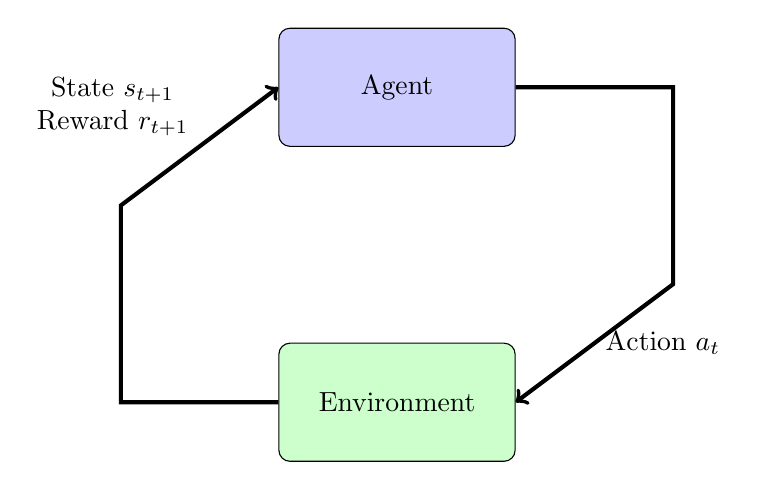
\begin{tikzpicture}[scale=1.0, every node/.style={scale=1.0}]
            % Agent
            \node[draw, rounded corners, fill=blue!20, minimum width=3cm, minimum height=1.5cm] (agent) at (0,2) {Agent};
            % Environment
            \node[draw, rounded corners, fill=green!20, minimum width=3cm, minimum height=1.5cm] (env) at (0,-2) {Environment};

            % Arrows
            \draw[->, thick, line width=1.5pt] (agent.east) -- ++(2,0) -- ++(0,-2.5) -- (env.east) node[midway, right, align=center] {Action $a_t$};
            \draw[->, thick, line width=1.5pt] (env.west) -- ++(-2,0) -- ++(0,2.5) -- (agent.west) node[midway, left, align=center, yshift=0.5cm] {State $s_{t+1}$\\Reward $r_{t+1}$};
        \end{tikzpicture}
    \end{center}

    \vspace{0.3cm}
    \begin{center}
        \textit{The agent observes, acts, and learns from feedback}
    \end{center}
\end{frame}

%-----------------------------------------------
% Slide: History of RL
%-----------------------------------------------
\begin{frame}{History of Reinforcement Learning}
    \begin{itemize}
        \item \textbf{1950s} -- Bellman: Dynamic Programming, Bellman Equation
        \item \textbf{1988} -- Sutton: Temporal Difference (TD) Learning
        \item \textbf{1989} -- Watkins: Q-Learning algorithm
        \item \textbf{1992} -- Tesauro: TD-Gammon (Backgammon)
        \item \textbf{2013} -- Mnih et al.: Deep Q-Network (DQN) plays Atari
        \item \textbf{2016} -- DeepMind: AlphaGo defeats world champion
        \item \textbf{2019} -- OpenAI Five: Beats world champions at Dota 2
        \item \textbf{2022+} -- RLHF: Training large language models
    \end{itemize}
\end{frame}

%-----------------------------------------------
% Slide: Roadmap
%-----------------------------------------------
\begin{frame}{Today's Roadmap}
    \begin{enumerate}
        \item \textbf{Introduction} -- What is RL? (You are here)
        \item \textbf{Game \& Agent Foundations} -- Snake as MDP
        \item \textbf{Algorithms} -- DQN, PPO, and training
        \item \textbf{Feature Engineering} -- State representations
        \item \textbf{???} -- Something challenging...
        \item \textbf{Conclusion} -- Limitations and future development
    \end{enumerate}
\end{frame}

%===============================================
% PRESENTER 2: Game & Agent Foundations
%===============================================
\presentertitle{2}{Game \& Agent Foundations}

%-----------------------------------------------
% Slide: What is an MDP?
%-----------------------------------------------
\begin{frame}{Markov Decision Process (MDP)}
    \textbf{Mathematical framework for sequential decision making}

    \vspace{0.5cm}
    An MDP is defined by a tuple $(S, A, P, R, \gamma)$:
    \begin{itemize}
        \item $S$ -- Set of \textbf{states} (all possible situations)
        \item $A$ -- Set of \textbf{actions} (what agent can do)
        \item $P(s'|s,a)$ -- \textbf{Transition probability} (dynamics)
        \item $R(s,a,s')$ -- \textbf{Reward function} (feedback)
        \item $\gamma \in [0,1]$ -- \textbf{Discount factor} (future importance)
    \end{itemize}
\end{frame}

%-----------------------------------------------
% Slide: The Agent-Environment Loop
%-----------------------------------------------
\begin{frame}{The Agent-Environment Loop}
    \textbf{A trajectory of experience:}

    \vspace{0.5cm}
    \begin{center}
        $s_0 \xrightarrow{a_0} r_0, s_1 \xrightarrow{a_1} r_1, s_2 \xrightarrow{a_2} r_2, s_3 \xrightarrow{a_3} \cdots$
    \end{center}

    \vspace{0.5cm}
    \begin{center}
        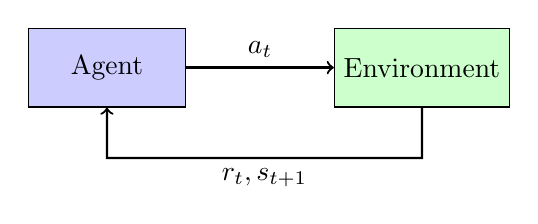
\begin{tikzpicture}[scale=0.8]
            % Agent
            \node[draw, rectangle, fill=blue!20, minimum width=2cm, minimum height=1cm] (agent) at (0,0) {Agent};
            % Environment
            \node[draw, rectangle, fill=green!20, minimum width=2cm, minimum height=1cm] (env) at (5,0) {Environment};

            % Arrows
            \draw[->, thick] (agent.east) -- node[above] {$a_t$} (env.west);
            \draw[->, thick] (env.south) -- ++(0,-0.8) -- node[below] {$r_t, s_{t+1}$} ++(-5,0) -- (agent.south);
        \end{tikzpicture}
    \end{center}

    \vspace{0.5cm}
    \textbf{Goal:} Find actions that maximize cumulative reward
    \[
    G_t = r_t + \gamma r_{t+1} + \gamma^2 r_{t+2} + \cdots = \sum_{k=0}^{\infty} \gamma^k r_{t+k}
    \]
\end{frame}

%-----------------------------------------------
% Slide: Snake Game Introduction
%-----------------------------------------------
\begin{frame}{The Snake Game}
    \begin{columns}
        \begin{column}{0.5\textwidth}
            \textbf{Rules:}
            \begin{itemize}
                \item Snake moves continuously
                \item Eating food makes snake grow
                \item Game ends on collision
            \end{itemize}

        \end{column}

        \begin{column}{0.5\textwidth}
            \begin{center}
                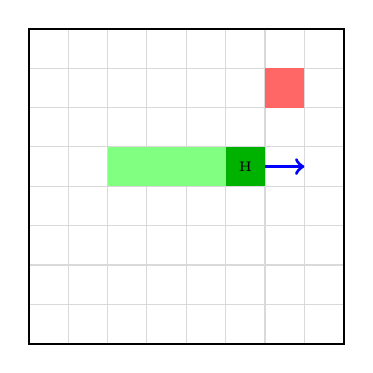
\begin{tikzpicture}[scale=0.5]
                    \draw[gray!30] (0,0) grid (8,8);
                    \draw[black, thick] (0,0) rectangle (8,8);

                    % Snake
                    \fill[green!50] (2,4) rectangle (3,5);
                    \fill[green!50] (3,4) rectangle (4,5);
                    \fill[green!50] (4,4) rectangle (5,5);
                    \fill[green!70!black] (5,4) rectangle (6,5);
                    \node at (5.5,4.5) {\tiny H};

                    % Food
                    \fill[red!60] (6,6) rectangle (7,7);

                    % Direction arrow
                    \draw[->, blue, very thick] (6,4.5) -- (7,4.5);
                \end{tikzpicture}
            \end{center}
        \end{column}
    \end{columns}
\end{frame}

%-----------------------------------------------
% Slide: Snake MDP - State Space
%-----------------------------------------------
\begin{frame}{Snake as MDP: State Space (Attempt 1)}
    \textbf{What information defines the current situation?}

    \vspace{0.5cm}
    \begin{columns}
        \begin{column}{0.5\textwidth}
            \begin{itemize}
                \item Grid size (e.g., 10x10)
                \item Snake head position $(x, y)$
                \item Snake body positions
                \item Food location $(f_x, f_y)$
            \end{itemize}

            \vspace{0.3cm}
            {\color{red} Is this enough?}
        \end{column}

        \begin{column}{0.5\textwidth}
            \begin{center}
                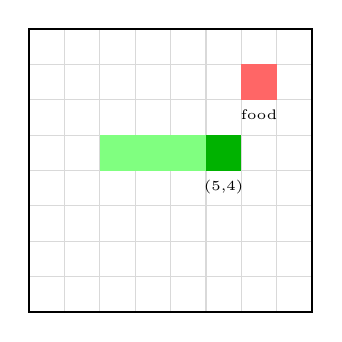
\begin{tikzpicture}[scale=0.45]
                    \draw[gray!30] (0,0) grid (8,8);
                    \draw[black, thick] (0,0) rectangle (8,8);

                    % Snake with labels
                    \fill[green!50] (2,4) rectangle (3,5);
                    \fill[green!50] (3,4) rectangle (4,5);
                    \fill[green!50] (4,4) rectangle (5,5);
                    \fill[green!70!black] (5,4) rectangle (6,5);

                    % Food
                    \fill[red!60] (6,6) rectangle (7,7);

                    % Labels
                    \node[below] at (5.5,4) {\tiny (5,4)};
                    \node[below] at (6.5,6) {\tiny food};
                \end{tikzpicture}
            \end{center}
        \end{column}
    \end{columns}
\end{frame}

%-----------------------------------------------
% Slide: Markov Property
%-----------------------------------------------
\begin{frame}{The Markov Property}
    \textbf{Key requirement for MDPs:}

    \vspace{0.5cm}
    \begin{center}
        \textit{``The future depends only on the present, not the past''}
    \end{center}

    \vspace{0.5cm}
    \[
    P(s_{t+1} | s_t, a_t) = P(s_{t+1} | s_t, a_t, s_{t-1}, a_{t-1}, \ldots)
    \]

    \vspace{0.5cm}
    \textbf{Problem with our state:}
    \begin{itemize}
        \item Same position can have different valid moves
        \item Which way is the snake facing?
        \item Without direction, we can't predict the next state!
    \end{itemize}

    \vspace{0.3cm}
    \begin{center}
        \fbox{State must contain ALL information needed for decision}
    \end{center}
\end{frame}

%-----------------------------------------------
% Slide: Snake MDP - State Space (Complete)
%-----------------------------------------------
\begin{frame}{Snake as MDP: State Space (Complete)}
    \textbf{Adding current direction to satisfy Markov property:}

    \vspace{0.5cm}
    \begin{columns}
        \begin{column}{0.5\textwidth}
            \begin{itemize}
                \item Grid size (e.g., 10x10)
                \item Snake head position $(x, y)$
                \item Snake body positions
                \item {\color{green!50!black} \textbf{Current direction}}
                \item Food location $(f_x, f_y)$
            \end{itemize}

            \vspace{0.3cm}
            {\color{green!50!black} Now the state is complete!}
        \end{column}

        \begin{column}{0.5\textwidth}
            \begin{center}
                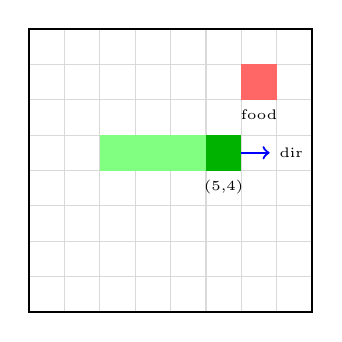
\begin{tikzpicture}[scale=0.45]
                    \draw[gray!30] (0,0) grid (8,8);
                    \draw[black, thick] (0,0) rectangle (8,8);

                    % Snake with labels
                    \fill[green!50] (2,4) rectangle (3,5);
                    \fill[green!50] (3,4) rectangle (4,5);
                    \fill[green!50] (4,4) rectangle (5,5);
                    \fill[green!70!black] (5,4) rectangle (6,5);

                    % Food
                    \fill[red!60] (6,6) rectangle (7,7);

                    % Labels
                    \node[below] at (5.5,4) {\tiny (5,4)};
                    \node[below] at (6.5,6) {\tiny food};
                    \draw[->, blue, thick] (6,4.5) -- (6.8,4.5);
                    \node[right] at (6.8,4.5) {\tiny dir};
                \end{tikzpicture}
            \end{center}
        \end{column}
    \end{columns}
\end{frame}

%-----------------------------------------------
% Slide: Snake MDP - Action Space
%-----------------------------------------------
\begin{frame}{Snake as MDP: Action Space}
    \textbf{What can the agent do?}

    \vspace{0.3cm}
    \begin{columns}
        \begin{column}{0.48\textwidth}
            \centering
            \textbf{Absolute (4 actions)}

            \vspace{0.2cm}
            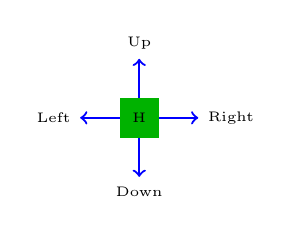
\begin{tikzpicture}[scale=0.5]
                % Snake head
                \fill[green!70!black] (2,2) rectangle (3,3);
                \node at (2.5,2.5) {\tiny H};

                % Action arrows
                \draw[->, blue, thick] (3,2.5) -- (4,2.5);
                \node[right] at (4,2.5) {\tiny Right};

                \draw[->, blue, thick] (2,2.5) -- (1,2.5);
                \node[left] at (1,2.5) {\tiny Left};

                \draw[->, blue, thick] (2.5,3) -- (2.5,4);
                \node[above] at (2.5,4) {\tiny Up};

                \draw[->, blue, thick] (2.5,2) -- (2.5,1);
                \node[below] at (2.5,1) {\tiny Down};
            \end{tikzpicture}

            \vspace{0.2cm}
            {\small Up, Down, Left, Right}

            {\footnotesize One action always = death}
        \end{column}

        \begin{column}{0.48\textwidth}
            \centering
            \textbf{Relative (3 actions)} {\color{green!50!black} $\checkmark$}

            \vspace{0.2cm}
            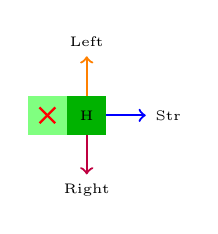
\begin{tikzpicture}[scale=0.5]
                % Snake head
                \fill[green!70!black] (2,2) rectangle (3,3);
                \node at (2.5,2.5) {\tiny H};

                % Body behind
                \fill[green!50] (1,2) rectangle (2,3);

                % Action arrows
                \draw[->, blue, thick] (3,2.5) -- (4,2.5);
                \node[right] at (4,2.5) {\tiny Str};

                \draw[->, orange, thick] (2.5,3) -- (2.5,4);
                \node[above] at (2.5,4) {\tiny Left};

                \draw[->, purple, thick] (2.5,2) -- (2.5,1);
                \node[below] at (2.5,1) {\tiny Right};

                % X for backward
                \draw[red, thick] (1.3,2.3) -- (1.7,2.7);
                \draw[red, thick] (1.3,2.7) -- (1.7,2.3);
            \end{tikzpicture}

            \vspace{0.2cm}
            {\small Straight, Left, Right}

            {\footnotesize No invalid actions}
        \end{column}
    \end{columns}

    \vspace{0.3cm}
    \begin{center}
        \fbox{We use relative actions: $|A| = 3$}
    \end{center}
\end{frame}

%-----------------------------------------------
% Slide: Snake MDP - Rewards
%-----------------------------------------------
\begin{frame}{Snake as MDP: Reward Function}
    \textbf{What feedback does the agent receive?}

    \vspace{0.5cm}
    \begin{center}
        \begin{tabular}{lc}
            \toprule
            \textbf{Event} & \textbf{Reward} \\
            \midrule
            Eat food & $+10$ \\
            Hit wall & $-10$ \\
            Hit self & $-10$ \\
            Each step & $-0.01$ (small penalty) \\
            \bottomrule
        \end{tabular}
    \end{center}

    \vspace{0.5cm}
    \textbf{Why step penalty?}
    \begin{itemize}
        \item Encourages efficiency
        \item Prevents infinite loops
        \item Balances exploration vs exploitation
    \end{itemize}
\end{frame}

%-----------------------------------------------
% Slide: Snake MDP - Terminal States
%-----------------------------------------------
\begin{frame}{Snake as MDP: Terminal States}
    \textbf{When does the episode end?}

    \vspace{0.5cm}
    \begin{columns}
        \begin{column}{0.5\textwidth}
            \textbf{Wall Collision:}
            \begin{center}
                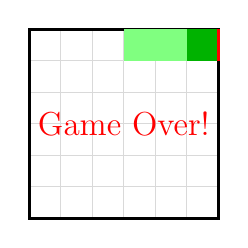
\begin{tikzpicture}[scale=0.4]
                    \draw[gray!30] (0,0) grid (6,6);
                    \draw[black, very thick] (0,0) rectangle (6,6);
                    \fill[green!50] (3,5) rectangle (4,6);
                    \fill[green!50] (4,5) rectangle (5,6);
                    \fill[green!70!black] (5,5) rectangle (6,6);
                    \draw[red, very thick] (6,5) -- (6,6);
                    \node[red] at (3,3) {\large Game Over!};
                \end{tikzpicture}
            \end{center}
        \end{column}

        \begin{column}{0.5\textwidth}
            \textbf{Self Collision:}
            \begin{center}
                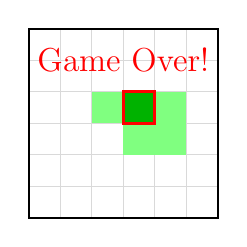
\begin{tikzpicture}[scale=0.4]
                    \draw[gray!30] (0,0) grid (6,6);
                    \draw[black, thick] (0,0) rectangle (6,6);
                    % Snake eating itself
                    \fill[green!50] (2,3) rectangle (3,4);
                    \fill[green!50] (3,3) rectangle (4,4);
                    \fill[green!50] (4,3) rectangle (5,4);
                    \fill[green!50] (4,2) rectangle (5,3);
                    \fill[green!50] (3,2) rectangle (4,3);
                    \fill[green!70!black] (3,3) rectangle (4,4);
                    \draw[red, very thick] (3,3) rectangle (4,4);
                    \node[red] at (3,5) {\large Game Over!};
                \end{tikzpicture}
            \end{center}
        \end{column}
    \end{columns}
\end{frame}

%-----------------------------------------------
% Slide: Policy
%-----------------------------------------------
\begin{frame}{Policy Function $\pi$}
    \textbf{The agent's developing strategy}

    \vspace{0.5cm}
    A policy $\pi$ maps states to actions:
    \[
    \pi: S \rightarrow A \quad \text{or} \quad \pi(a|s) = P(a_t = a | s_t = s)
    \]

    \vspace{0.5cm}
    \begin{itemize}
        \item \textbf{Deterministic:} $\pi(s) = a$ (one action per state)
        \item \textbf{Stochastic:} $\pi(a|s)$ (probability distribution over actions)
    \end{itemize}

    \vspace{0.5cm}
    \begin{center}
        \fbox{Goal of RL: Find the \textbf{optimal policy} $\pi^*$}
    \end{center}
\end{frame}

%-----------------------------------------------
% Slide: Policy Example
%-----------------------------------------------
\begin{frame}{Policy in Action}
    \begin{columns}
        \begin{column}{0.5\textwidth}
            \begin{center}
                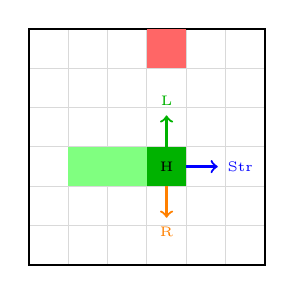
\begin{tikzpicture}[scale=0.5]
                    \draw[gray!30] (0,0) grid (6,6);
                    \draw[black, thick] (0,0) rectangle (6,6);

                    % Snake body
                    \fill[green!50] (1,2) rectangle (2,3);
                    \fill[green!50] (2,2) rectangle (3,3);
                    \fill[green!70!black] (3,2) rectangle (4,3);
                    \node at (3.5,2.5) {\tiny H};

                    % Food (on the Left side - up from snake's perspective)
                    \fill[red!60] (3,5) rectangle (4,6);

                    % Action arrows from head
                    \draw[->, blue, thick] (4,2.5) -- (4.8,2.5);
                    \node[right, blue] at (4.8,2.5) {\tiny Str};
                    \draw[->, green!70!black, thick] (3.5,3) -- (3.5,3.8);
                    \node[above, green!70!black] at (3.5,3.8) {\tiny L};
                    \draw[->, orange, thick] (3.5,2) -- (3.5,1.2);
                    \node[below, orange] at (3.5,1.2) {\tiny R};
                \end{tikzpicture}

                \vspace{0.3cm}
                {\small Current state $s$}
            \end{center}
        \end{column}

        \begin{column}{0.5\textwidth}
            \begin{center}
                $\pi(a|s)$:

                \vspace{0.3cm}
                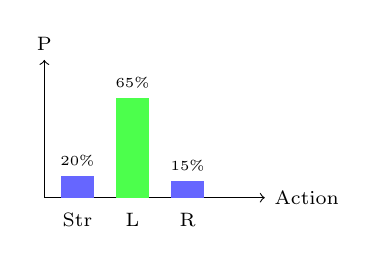
\begin{tikzpicture}[scale=0.7]
                    % Axes
                    \draw[->] (0,0) -- (4,0) node[right] {\scriptsize Action};
                    \draw[->] (0,0) -- (0,2.5) node[above] {\scriptsize P};
                    % Bars
                    \fill[blue!60] (0.3,0) rectangle (0.9,0.4);
                    \fill[green!70] (1.3,0) rectangle (1.9,1.8);
                    \fill[blue!60] (2.3,0) rectangle (2.9,0.3);
                    % Labels
                    \node[below] at (0.6,-0.1) {\scriptsize Str};
                    \node[below] at (1.6,-0.1) {\scriptsize L};
                    \node[below] at (2.6,-0.1) {\scriptsize R};
                    % Probabilities
                    \node[above] at (0.6,0.4) {\tiny 20\%};
                    \node[above] at (1.6,1.8) {\tiny 65\%};
                    \node[above] at (2.6,0.3) {\tiny 15\%};
                \end{tikzpicture}

                \vspace{0.3cm}
                {\small Left has highest probability}\\
                {\small (food is up-right)}
            \end{center}
        \end{column}
    \end{columns}
\end{frame}

%-----------------------------------------------
% Slide: State-Value Function
%-----------------------------------------------
\begin{frame}{State-Value Function $V(s)$}
    \textbf{How good is it to \textit{be} in state $s$?}

    \vspace{0.5cm}
    \[
    V^\pi(s) = \mathbb{E}_\pi\left[ G_t \mid s_t = s \right] = \mathbb{E}_\pi\left[ \sum_{k=0}^{\infty} \gamma^k r_{t+k} \mid s_t = s \right]
    \]

    \vspace{0.5cm}
    \begin{itemize}
        \item Expected cumulative reward starting from state $s$
        \item Following policy $\pi$
    \end{itemize}

    \vspace{0.5cm}
    \begin{center}
        \textit{``If I'm in this state, how much reward can I expect?''}
    \end{center}
\end{frame}

%-----------------------------------------------
% Slide: State-Value Example
%-----------------------------------------------
\begin{frame}{State Values in Snake}
    \begin{center}
        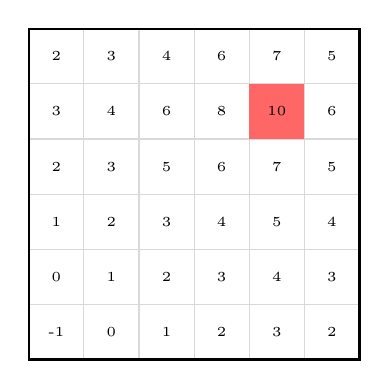
\begin{tikzpicture}[scale=0.7]
            \draw[gray!30] (0,0) grid (6,6);
            \draw[black, thick] (0,0) rectangle (6,6);

            % Food
            \fill[red!60] (4,4) rectangle (5,5);

            % Value labels in cells (higher near food)
            \node at (0.5,5.5) {\tiny 2};
            \node at (1.5,5.5) {\tiny 3};
            \node at (2.5,5.5) {\tiny 4};
            \node at (3.5,5.5) {\tiny 6};
            \node at (4.5,5.5) {\tiny 7};
            \node at (5.5,5.5) {\tiny 5};

            \node at (0.5,4.5) {\tiny 3};
            \node at (1.5,4.5) {\tiny 4};
            \node at (2.5,4.5) {\tiny 6};
            \node at (3.5,4.5) {\tiny 8};
            \node at (4.5,4.5) {\tiny 10};
            \node at (5.5,4.5) {\tiny 6};

            \node at (0.5,3.5) {\tiny 2};
            \node at (1.5,3.5) {\tiny 3};
            \node at (2.5,3.5) {\tiny 5};
            \node at (3.5,3.5) {\tiny 6};
            \node at (4.5,3.5) {\tiny 7};
            \node at (5.5,3.5) {\tiny 5};

            \node at (0.5,2.5) {\tiny 1};
            \node at (1.5,2.5) {\tiny 2};
            \node at (2.5,2.5) {\tiny 3};
            \node at (3.5,2.5) {\tiny 4};
            \node at (4.5,2.5) {\tiny 5};
            \node at (5.5,2.5) {\tiny 4};

            \node at (0.5,1.5) {\tiny 0};
            \node at (1.5,1.5) {\tiny 1};
            \node at (2.5,1.5) {\tiny 2};
            \node at (3.5,1.5) {\tiny 3};
            \node at (4.5,1.5) {\tiny 4};
            \node at (5.5,1.5) {\tiny 3};

            \node at (0.5,0.5) {\tiny -1};
            \node at (1.5,0.5) {\tiny 0};
            \node at (2.5,0.5) {\tiny 1};
            \node at (3.5,0.5) {\tiny 2};
            \node at (4.5,0.5) {\tiny 3};
            \node at (5.5,0.5) {\tiny 2};
        \end{tikzpicture}

        \vspace{0.5cm}
        {\small Values increase closer to food}\\
        {\small $V(s)$ guides the agent toward rewards}
    \end{center}
\end{frame}

%-----------------------------------------------
% Slide: Action-Value Function
%-----------------------------------------------
\begin{frame}{Action-Value Function $Q(s,a)$}
    \textbf{How good is it to \textit{take action} $a$ in state $s$?}

    \vspace{0.5cm}
    \[
    Q^\pi(s,a) = \mathbb{E}_\pi\left[ G_t \mid s_t = s, a_t = a \right]
    \]

    \vspace{0.5cm}
    \begin{itemize}
        \item Expected cumulative reward after taking action $a$ in state $s$
        \item Then following policy $\pi$
    \end{itemize}

    \vspace{0.5cm}
    \begin{center}
        \textit{``If I take this action here, how much reward can I expect?''}
    \end{center}

    \vspace{0.3cm}
    \begin{center}
        \fbox{This is what DQN learns!}
    \end{center}
\end{frame}

%-----------------------------------------------
% Slide: From Q to Policy
%-----------------------------------------------
\begin{frame}{From Q-Values to Policy}
    \begin{center}
        \textbf{The policy uses Q-values to decide action probabilities}
    \end{center}

    \vspace{0.5cm}
    \begin{columns}
        \begin{column}{0.5\textwidth}
            \begin{center}
                \textbf{Q-values for state $s$:}

                \vspace{0.3cm}
                \begin{tabular}{lc}
                    $Q(s, \text{Straight})$ & $= 3$ \\
                    $Q(s, \text{Left})$ & $= 8$ \\
                    $Q(s, \text{Right})$ & $= 2$ \\
                \end{tabular}
            \end{center}
        \end{column}

        \begin{column}{0.1\textwidth}
            \begin{center}
                $\Rightarrow$
            \end{center}
        \end{column}

        \begin{column}{0.4\textwidth}
            \begin{center}
                \textbf{Policy $\pi(a|s)$:}

                \vspace{0.3cm}
                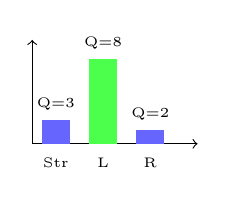
\begin{tikzpicture}[scale=0.6]
                    \draw[->] (0,0) -- (3.5,0);
                    \draw[->] (0,0) -- (0,2.2);
                    \fill[blue!60] (0.2,0) rectangle (0.8,0.5);
                    \fill[green!70] (1.2,0) rectangle (1.8,1.8);
                    \fill[blue!60] (2.2,0) rectangle (2.8,0.3);
                    \node[below] at (0.5,-0.1) {\tiny Str};
                    \node[below] at (1.5,-0.1) {\tiny L};
                    \node[below] at (2.5,-0.1) {\tiny R};
                    % Q-values above bars
                    \node[above] at (0.5,0.5) {\tiny Q=3};
                    \node[above] at (1.5,1.8) {\tiny Q=8};
                    \node[above] at (2.5,0.3) {\tiny Q=2};
                \end{tikzpicture}
            \end{center}
        \end{column}
    \end{columns}

    \vspace{0.5cm}
    \begin{center}
        \fbox{Higher Q-value $\rightarrow$ Higher probability}
    \end{center}
\end{frame}

%-----------------------------------------------
% Slide: Policy-Q Cycle
%-----------------------------------------------
\begin{frame}{The Learning Cycle}
    \begin{center}
        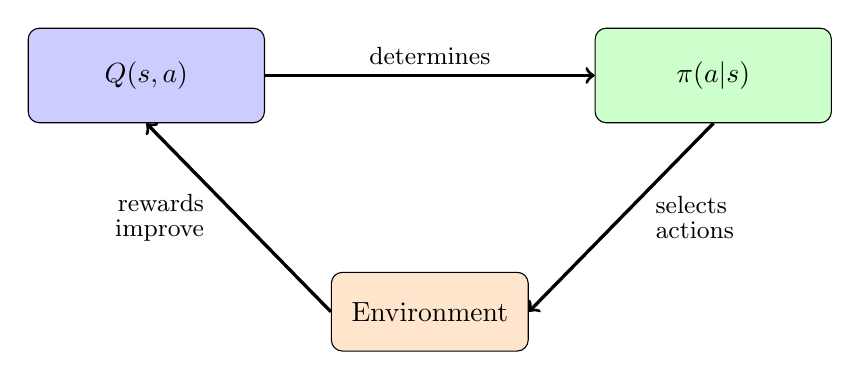
\begin{tikzpicture}[scale=1.2]
            % Nodes
            \node[draw, rectangle, rounded corners, fill=blue!20, minimum width=3cm, minimum height=1.2cm] (Q) at (0,0) {$Q(s,a)$};
            \node[draw, rectangle, rounded corners, fill=green!20, minimum width=3cm, minimum height=1.2cm] (pi) at (6,0) {$\pi(a|s)$};
            \node[draw, rectangle, rounded corners, fill=orange!20, minimum width=2.5cm, minimum height=1cm] (env) at (3,-2.5) {Environment};

            % Arrows
            \draw[->, very thick] (Q.east) -- node[above] {\small determines} (pi.west);
            \draw[->, very thick] (pi.south) -- node[right, align=left, xshift=0.3cm] {\small selects\\[-0.1cm]\small actions} (env.east);
            \draw[->, very thick] (env.west) -- node[left, align=right, xshift=-0.3cm] {\small rewards\\[-0.1cm]\small improve} (Q.south);
        \end{tikzpicture}

        \vspace{0.8cm}
        \begin{enumerate}
            \item Q-function estimates action values
            \item Policy uses Q to select actions
            \item Environment gives rewards
            \item Rewards update Q-function
        \end{enumerate}
    \end{center}
\end{frame}

%-----------------------------------------------
% Slide: Bellman Equation
%-----------------------------------------------
\begin{frame}{Bellman Equation}
    \begin{center}
        {\large The recursive relationship that makes RL possible}
    \end{center}

    \vspace{0.5cm}
    \[
    Q^*(s,a) = R(s,a) + \gamma \max_{a'} Q^*(s',a')
    \]

    \vspace{0.5cm}
    \begin{itemize}
        \item $R(s,a)$ = immediate reward
        \item $\gamma$ = discount factor (importance of future)
        \item $\max_{a'} Q^*(s',a')$ = best future value
    \end{itemize}

    \vspace{0.3cm}
    \begin{center}
        \textit{``The value now depends on the value later''}
    \end{center}
\end{frame}

%===============================================
% PRESENTER 3: Building the Snake Agent
%===============================================
\presentertitle{3}{Building the Snake Agent}

%-----------------------------------------------
% Slide: Q-Learning
%-----------------------------------------------
\begin{frame}{Q-Learning}
    \textbf{Update rule:}
    \[
    Q(s,a) \leftarrow Q(s,a) + \underbrace{\alpha}_{\text{learning rate}} \left[ \underbrace{r + \gamma \max_{a'} Q(s', a')}_{\text{TD target}} - Q(s,a) \right]
    \]

    \vspace{1cm}
    \textbf{Problem:} Q-table doesn't scale to large state spaces!
\end{frame}

%-----------------------------------------------
% Slide: Training a Neural Network for RL
%-----------------------------------------------
\begin{frame}{Training a Neural Network for RL}
    \textbf{Loss Function:}

    \vspace{1cm}
    \[
    L = \left( \underbrace{Q_\theta(s,a)}_{\text{predicted}} - \underbrace{(r + \gamma \max_{a'} Q(s',a'))}_{\text{TD target}} \right)^2
    \]

    \vspace{1cm}
    \begin{center}
        \textit{No labels needed -- the target comes from the Bellman equation!}
    \end{center}
\end{frame}

%-----------------------------------------------
% Slide: Deep Q-Networks (DQN)
%-----------------------------------------------
\begin{frame}{Deep Q-Networks (DQN)}
    \textbf{Solution:} Use neural network to approximate Q(s,a)

    \vspace{0.5cm}
    \begin{center}
        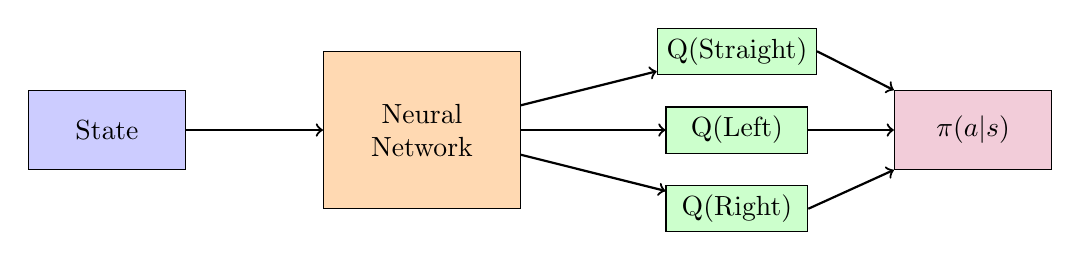
\begin{tikzpicture}[scale=1.0]
            % Input
            \node[draw, rectangle, fill=blue!20, minimum width=2cm, minimum height=1cm] (input) at (0,0) {State};
            % Network
            \node[draw, rectangle, fill=orange!30, minimum width=2.5cm, minimum height=2cm, align=center] (nn) at (4,0) {Neural\\Network};
            % Outputs (3 actions: straight, left, right)
            \node[draw, rectangle, fill=green!20, minimum width=1.8cm] (q1) at (8,1) {Q(Straight)};
            \node[draw, rectangle, fill=green!20, minimum width=1.8cm] (q2) at (8,0) {Q(Left)};
            \node[draw, rectangle, fill=green!20, minimum width=1.8cm] (q3) at (8,-1) {Q(Right)};
            % Policy
            \node[draw, rectangle, fill=purple!20, minimum width=2cm, minimum height=1cm] (policy) at (11,0) {$\pi(a|s)$};

            % Arrows
            \draw[->, thick] (input) -- (nn);
            \draw[->, thick] (nn) -- (q1);
            \draw[->, thick] (nn) -- (q2);
            \draw[->, thick] (nn) -- (q3);
            \draw[->, thick] (q1.east) -- (policy.north west);
            \draw[->, thick] (q2.east) -- (policy.west);
            \draw[->, thick] (q3.east) -- (policy.south west);
        \end{tikzpicture}
    \end{center}
\end{frame}

%-----------------------------------------------
% Slide: Exploration vs. Exploitation
%-----------------------------------------------
\begin{frame}{Exploration vs. Exploitation}
    \begin{center}
        \textit{The agent found food going right. Should it always go right?}
    \end{center}

    \vspace{0.5cm}
    \begin{columns}[T]
        \begin{column}{0.48\textwidth}
            \centering
            \textbf{Exploration}

            \vspace{0.3cm}
            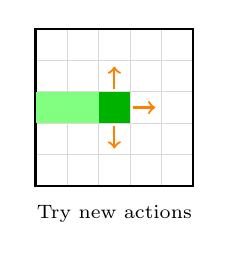
\begin{tikzpicture}[scale=0.4]
                % Grid
                \draw[gray!30] (0,0) grid (5,5);
                \draw[black, thick] (0,0) rectangle (5,5);
                % Snake body
                \fill[green!50] (0,2) rectangle (1,3);
                \fill[green!50] (1,2) rectangle (2,3);
                % Snake head
                \fill[green!70!black] (2,2) rectangle (3,3);
                % Arrows in multiple directions
                \draw[->, thick, orange] (2.5,3.1) -- (2.5,3.8);
                \draw[->, thick, orange] (3.1,2.5) -- (3.8,2.5);
                \draw[->, thick, orange] (2.5,1.9) -- (2.5,1.2);
                \node[below] at (2.5,-0.3) {\scriptsize Try new actions};
            \end{tikzpicture}

            \vspace{0.3cm}
            Discover better strategies
        \end{column}

        \begin{column}{0.48\textwidth}
            \centering
            \textbf{Exploitation}

            \vspace{0.3cm}
            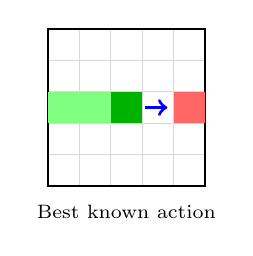
\begin{tikzpicture}[scale=0.4]
                % Grid
                \draw[gray!30] (0,0) grid (5,5);
                \draw[black, thick] (0,0) rectangle (5,5);
                % Snake body
                \fill[green!50] (0,2) rectangle (1,3);
                \fill[green!50] (1,2) rectangle (2,3);
                % Snake head
                \fill[green!70!black] (2,2) rectangle (3,3);
                % Food to the right
                \fill[red!60] (4,2) rectangle (5,3);
                % Arrow right (best known action)
                \draw[->, very thick, blue] (3.1,2.5) -- (3.8,2.5);
                \node[below] at (2.5,-0.3) {\scriptsize Best known action};
            \end{tikzpicture}

            \vspace{0.3cm}
            Use current knowledge
        \end{column}
    \end{columns}

    \vspace{0.5cm}
    \begin{center}
        \fbox{Balance is key: too much exploration = slow; too little = suboptimal}
    \end{center}
\end{frame}

%-----------------------------------------------
% Slide: Epsilon-Greedy Strategy
%-----------------------------------------------
\begin{frame}{$\epsilon$-Greedy Strategy}
    \begin{columns}[T]
        \begin{column}{0.48\textwidth}
            \centering
            \textbf{High $\epsilon$ = 0.75} (Early training)

            \vspace{0.3cm}
            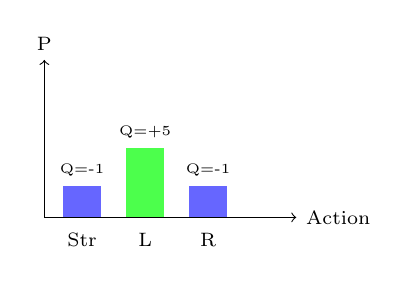
\begin{tikzpicture}[scale=0.8]
                % Axes
                \draw[->] (0,0) -- (4,0) node[right] {\scriptsize Action};
                \draw[->] (0,0) -- (0,2.5) node[above] {\scriptsize P};
                % Bars
                \fill[blue!60] (0.3,0) rectangle (0.9,0.5);
                \fill[green!70] (1.3,0) rectangle (1.9,1.1);
                \fill[blue!60] (2.3,0) rectangle (2.9,0.5);
                % Labels
                \node[below] at (0.6,-0.1) {\scriptsize Str};
                \node[below] at (1.6,-0.1) {\scriptsize L};
                \node[below] at (2.6,-0.1) {\scriptsize R};
                % Q-values above bars
                \node[above] at (0.6,0.5) {\tiny Q=-1};
                \node[above] at (1.6,1.1) {\tiny Q=+5};
                \node[above] at (2.6,0.5) {\tiny Q=-1};
            \end{tikzpicture}

            \vspace{0.2cm}
            {\small More exploration}
        \end{column}

        \begin{column}{0.48\textwidth}
            \centering
            \textbf{Low $\epsilon$ = 0.05} (Late training)

            \vspace{0.3cm}
            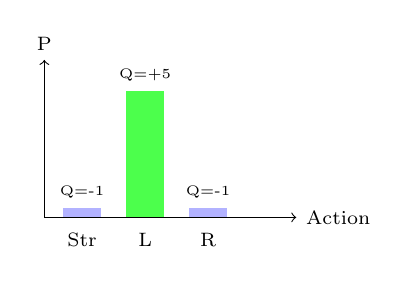
\begin{tikzpicture}[scale=0.8]
                % Axes
                \draw[->] (0,0) -- (4,0) node[right] {\scriptsize Action};
                \draw[->] (0,0) -- (0,2.5) node[above] {\scriptsize P};
                % Bars
                \fill[blue!30] (0.3,0) rectangle (0.9,0.15);
                \fill[green!70] (1.3,0) rectangle (1.9,2);
                \fill[blue!30] (2.3,0) rectangle (2.9,0.15);
                % Labels
                \node[below] at (0.6,-0.1) {\scriptsize Str};
                \node[below] at (1.6,-0.1) {\scriptsize L};
                \node[below] at (2.6,-0.1) {\scriptsize R};
                % Q-values above bars
                \node[above] at (0.6,0.15) {\tiny Q=-1};
                \node[above] at (1.6,2) {\tiny Q=+5};
                \node[above] at (2.6,0.15) {\tiny Q=-1};
            \end{tikzpicture}

            \vspace{0.2cm}
            {\small Best action dominates}
        \end{column}
    \end{columns}

    \vspace{0.5cm}
    \begin{center}
        \fbox{$\epsilon$: choose randomly $\epsilon \times 100$\% of the time}
    \end{center}
\end{frame}

%-----------------------------------------------
% Slide: Network Architecture: MLP vs CNN
%-----------------------------------------------
\begin{frame}{Network Architecture: MLP vs CNN}
    \begin{columns}[T]
        \begin{column}{0.48\textwidth}
            \centering
            \textbf{MLP (Feature Vector)}

            \vspace{0.3cm}
            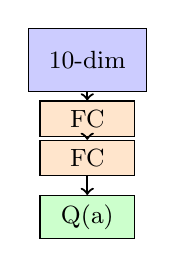
\begin{tikzpicture}[scale=0.5]
                % Input
                \node[draw, rectangle, fill=blue!20, minimum width=1.5cm, minimum height=0.8cm] (input) at (0,0) {\small 10-dim};
                % Hidden
                \node[draw, rectangle, fill=orange!20, minimum width=1.2cm] (h1) at (0,-1.5) {\small FC};
                \node[draw, rectangle, fill=orange!20, minimum width=1.2cm] (h2) at (0,-2.5) {\small FC};
                % Output
                \node[draw, rectangle, fill=green!20, minimum width=1.2cm] (out) at (0,-4) {\small Q(a)};

                \draw[->, thick] (input) -- (h1);
                \draw[->, thick] (h1) -- (h2);
                \draw[->, thick] (h2) -- (out);
            \end{tikzpicture}

            \vspace{0.3cm}
            {\small Hand-crafted features}

            {\footnotesize Fast training, interpretable}
        \end{column}

        \begin{column}{0.48\textwidth}
            \centering
            \textbf{CNN (Raw Grid)}

            \vspace{0.3cm}
            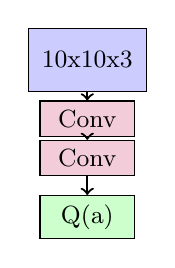
\begin{tikzpicture}[scale=0.5]
                % Input grid
                \node[draw, rectangle, fill=blue!20, minimum width=1.5cm, minimum height=0.8cm] (input) at (0,0) {\small 10x10x3};
                % Conv layers
                \node[draw, rectangle, fill=purple!20, minimum width=1.2cm] (c1) at (0,-1.5) {\small Conv};
                \node[draw, rectangle, fill=purple!20, minimum width=1.2cm] (c2) at (0,-2.5) {\small Conv};
                % Output
                \node[draw, rectangle, fill=green!20, minimum width=1.2cm] (out) at (0,-4) {\small Q(a)};

                \draw[->, thick] (input) -- (c1);
                \draw[->, thick] (c1) -- (c2);
                \draw[->, thick] (c2) -- (out);
            \end{tikzpicture}

            \vspace{0.3cm}
            {\small Learns features automatically}

            {\footnotesize Slower, more data needed}
        \end{column}
    \end{columns}

    \vspace{0.5cm}
    \begin{center}
        \textit{Both output Q-values -- only the input representation differs}
    \end{center}
\end{frame}

%-----------------------------------------------
% Slide: State Representation
%-----------------------------------------------
\begin{frame}{What Does the Agent See?}
    \textbf{The agent doesn't see the grid directly!}

    \vspace{0.5cm}
    We must convert the game state into a feature vector:
    \begin{itemize}
        \item Input to the neural network
        \item Must capture essential information
        \item Affects learning speed and performance
    \end{itemize}

    \vspace{0.5cm}
    \begin{center}
        Game State $\rightarrow$ \fbox{Feature Extraction} $\rightarrow$ Neural Network
    \end{center}
\end{frame}

%-----------------------------------------------
% Slide: Basic Features
%-----------------------------------------------
\begin{frame}{Basic Features (10 dimensions)}
    \begin{columns}
        \begin{column}{0.5\textwidth}
            \textbf{Direction (3 values) (MP):}
            \begin{itemize}
                \item One-hot encoding
            \end{itemize}

            \vspace{0.3cm}
            \textbf{Food Direction (4 values):}
            \begin{itemize}
                \item Relative to head
                \item food\_left, food\_right
                \item food\_up, food\_down
            \end{itemize}

            \vspace{0.3cm}
            \textbf{Danger Sensors (3 values):}
            \begin{itemize}
                \item danger\_straight
                \item danger\_left
                \item danger\_right
            \end{itemize}
        \end{column}

        \begin{column}{0.5\textwidth}
            \begin{center}
                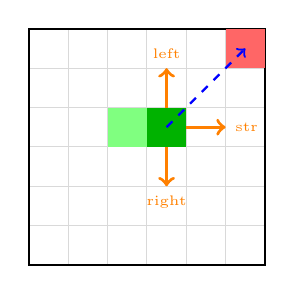
\begin{tikzpicture}[scale=0.5]
                    \draw[gray!30] (0,0) grid (6,6);
                    \draw[black, thick] (0,0) rectangle (6,6);

                    % Snake
                    \fill[green!50] (2,3) rectangle (3,4);
                    \fill[green!70!black] (3,3) rectangle (4,4);

                    % Food
                    \fill[red!60] (5,5) rectangle (6,6);

                    % Danger sensors
                    \draw[->, orange, very thick] (4,3.5) -- (5,3.5);
                    \node[right, orange] at (5,3.5) {\tiny str};
                    \draw[->, orange, very thick] (3.5,4) -- (3.5,5);
                    \node[above, orange] at (3.5,5) {\tiny left};
                    \draw[->, orange, very thick] (3.5,3) -- (3.5,2);
                    \node[below, orange] at (3.5,2) {\tiny right};

                    % Food direction
                    \draw[->, blue, dashed, thick] (3.5,3.5) -- (5.5,5.5);
                \end{tikzpicture}
            \end{center}
        \end{column}
    \end{columns}
\end{frame}

%-----------------------------------------------
% Slide: Basic Agent Demo
%-----------------------------------------------
\begin{frame}{Basic DQN Agent}
    \begin{center}
        \includegraphics[width=0.7\textwidth]{figures/training/dqn_basic_20251129_231638.png}

        \vspace{0.3cm}
        \textit{Trained with 10-dimensional feature vector}
    \end{center}
\end{frame}

%-----------------------------------------------
% Slide: Without Experience Replay
%-----------------------------------------------
\begin{frame}{Training Without Replay}
    \begin{center}
        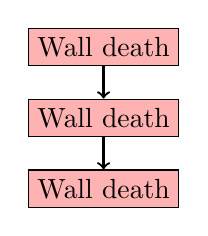
\begin{tikzpicture}[scale=0.6]
            % Sequential experiences
            \node[draw, rectangle, fill=red!30] (e1) at (0,0) {Wall death};
            \node[draw, rectangle, fill=red!30] (e2) at (0,-1.5) {Wall death};
            \node[draw, rectangle, fill=red!30] (e3) at (0,-3) {Wall death};
            \draw[->, thick] (e1) -- (e2);
            \draw[->, thick] (e2) -- (e3);
        \end{tikzpicture}

        \vspace{0.5cm}
        {\color{red} Only learns ``avoid walls''}\\
        Forgets how to get food!
    \end{center}
\end{frame}

%-----------------------------------------------
% Slide: With Experience Replay
%-----------------------------------------------
\begin{frame}{Training With Experience Replay}
    \begin{center}
        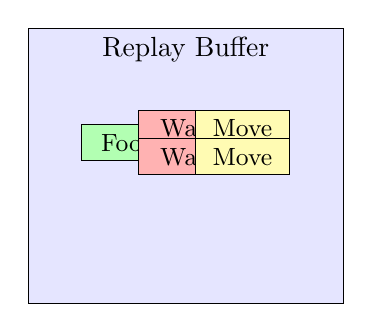
\begin{tikzpicture}[scale=0.6]
            % Buffer
            \node[draw, rectangle, fill=blue!10, minimum width=4cm, minimum height=3.5cm] (buf) at (0,0) {};
            \node[above] at (0,2) {Replay Buffer};
            % Food column
            \node[draw, rectangle, fill=green!30, minimum width=1.2cm] at (-1.2,0.5) {\small Food};
            % Wall column (stacked)
            \node[draw, rectangle, fill=red!30, minimum width=1.2cm] at (0,0.8) {\small Wall};
            \node[draw, rectangle, fill=red!30, minimum width=1.2cm] at (0,0.2) {\small Wall};
            % Move column (stacked)
            \node[draw, rectangle, fill=yellow!30, minimum width=1.2cm] at (1.2,0.8) {\small Move};
            \node[draw, rectangle, fill=yellow!30, minimum width=1.2cm] at (1.2,0.2) {\small Move};
        \end{tikzpicture}

        \vspace{0.5cm}
        {\color{green!50!black} Random sample from all}\\
        Learns everything together!
    \end{center}
\end{frame}

%-----------------------------------------------
% Slide: DQN Variants
%-----------------------------------------------
\begin{frame}{DQN Variants}
    \begin{itemize}
        \item \textbf{Double DQN} -- Reduces overestimation bias
        \vspace{0.3cm}
        \item \textbf{Dueling DQN} -- Separates value and advantage: $Q(s,a) = V(s) + A(s,a)$
        \vspace{0.3cm}
        \item \textbf{PER} -- Prioritized Experience Replay
        \vspace{0.3cm}
        \item \textbf{Noisy DQN} -- Adds noise for exploration
        \vspace{0.3cm}
        \item \textbf{Rainbow} -- Combines all improvements
    \end{itemize}
\end{frame}

%-----------------------------------------------
% Slide: Policy Gradient Methods
%-----------------------------------------------
\begin{frame}{Policy Gradient: PPO}
    \textbf{Different approach:} Directly optimize the policy $\pi(a|s)$

    \vspace{0.5cm}
    \textbf{PPO (Proximal Policy Optimization):}
    \begin{itemize}
        \item Actor-Critic architecture
        \item Clipped surrogate objective (stable updates)
        \item Most popular policy gradient method
    \end{itemize}

    \vspace{0.5cm}
    \begin{center}
        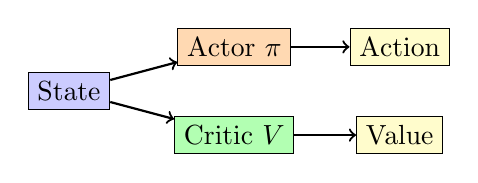
\begin{tikzpicture}[scale=0.7]
            \node[draw, rectangle, fill=blue!20] (state) at (0,0) {State};
            \node[draw, rectangle, fill=orange!30] (actor) at (3,0.8) {Actor $\pi$};
            \node[draw, rectangle, fill=green!30] (critic) at (3,-0.8) {Critic $V$};
            \node[draw, rectangle, fill=yellow!20] (action) at (6,0.8) {Action};
            \node[draw, rectangle, fill=yellow!20] (value) at (6,-0.8) {Value};

            \draw[->, thick] (state) -- (actor);
            \draw[->, thick] (state) -- (critic);
            \draw[->, thick] (actor) -- (action);
            \draw[->, thick] (critic) -- (value);
        \end{tikzpicture}
    \end{center}
\end{frame}

%-----------------------------------------------
% Slide: PPO Demo
%-----------------------------------------------
\begin{frame}{PPO Agent Demo}
    \begin{center}
        \includegraphics[width=0.7\textwidth]{figures/training/ppo_basic_20251129_231638.png}

        \vspace{0.3cm}
        \textit{PPO agent trained with basic features}
    \end{center}
\end{frame}

%===============================================
% PRESENTER 4: Feature Engineering
%===============================================
\presentertitle{4}{Feature Engineering}

%-----------------------------------------------
% Slide: Limitations of Basic Features
%-----------------------------------------------
\begin{frame}{Can We Do Better?}
    \textbf{Basic features work, but have limitations:}

    \vspace{0.5cm}
    \begin{itemize}
        \item Only sees immediate neighbors
        \item Cannot detect traps or dead-ends
        \item No awareness of available space
    \end{itemize}

    \vspace{0.5cm}
    \textbf{Let's explore better feature representations...}
\end{frame}

%-----------------------------------------------
% Slide: Death Causes Graph
%-----------------------------------------------
\begin{frame}{Why Do Agents Die?}
    \begin{center}
        \includegraphics[width=0.7\textwidth]{figures/training/double_dqn_basic_20251129_231638.png}

        \vspace{0.3cm}
        \textit{Most deaths come from self-collision (trapping)}
    \end{center}
\end{frame}

%-----------------------------------------------
% Slide: The Trapping Problem
%-----------------------------------------------
\begin{frame}{The Trapping Problem}
    \begin{columns}
        \begin{column}{0.5\textwidth}
            \begin{center}
                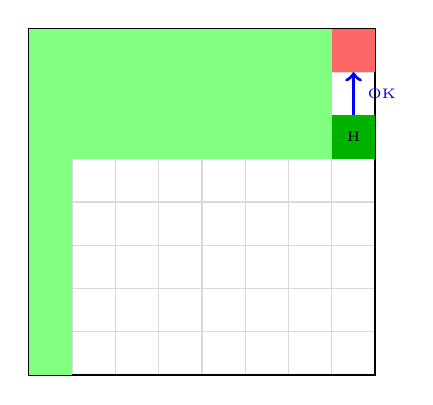
\begin{tikzpicture}[scale=0.55]
                    \draw[gray!30] (0,0) grid (8,8);
                    \draw[black, thick] (0,0) rectangle (8,8);

                    % Snake body forming L-shape trap
                    \fill[green!50] (0,0) rectangle (1,1);
                    \fill[green!50] (0,1) rectangle (1,2);
                    \fill[green!50] (0,2) rectangle (1,3);
                    \fill[green!50] (0,3) rectangle (1,4);
                    \fill[green!50] (0,4) rectangle (1,5);
                    \fill[green!50] (1,5) rectangle (2,6);
                    \fill[green!50] (2,5) rectangle (3,6);
                    \fill[green!50] (3,5) rectangle (4,6);
                    \fill[green!50] (4,5) rectangle (5,6);
                    \fill[green!50] (5,5) rectangle (6,6);
                    \fill[green!50] (6,5) rectangle (7,6);
                    \fill[green!70!black] (7,5) rectangle (8,6);
                    \node at (7.5,5.5) {\tiny H};

                    % Food in top right corner
                    \fill[red!60] (7,7) rectangle (8,8);

                    % Shade trapped area (same green as snake body)
                    \fill[green!50] (0,5) rectangle (1,8);
                    \fill[green!50] (1,6) rectangle (7,8);

                    % Danger sensors (all clear!)
                    \draw[->, blue, very thick] (7.5,6) -- (7.5,7);
                    \node[blue, right] at (7.6,6.5) {\tiny OK};
                \end{tikzpicture}
            \end{center}
        \end{column}

        \begin{column}{0.5\textwidth}
            \textbf{What basic features see:}
            \begin{itemize}
                \item danger\_straight = 1 \checkmark
                \item danger\_left = 0 \checkmark
                \item danger\_right = 0 \checkmark
                \item food\_left = 1 \checkmark
            \end{itemize}

            \vspace{0.3cm}
            \textbf{Reality:}
            \begin{itemize}
                \item {\color{red} Only 3 cells reachable!}
                \item Going left leads to death
            \end{itemize}

            \vspace{0.3cm}
            \fbox{Agent can't see the trap}
        \end{column}
    \end{columns}
\end{frame}

%-----------------------------------------------
% Slide: Flood-Fill Features
%-----------------------------------------------
\begin{frame}{Flood-Fill Features (13 dimensions)}
    \textbf{Solution:} Add reachable space information

    \vspace{0.5cm}
    \begin{columns}
        \begin{column}{0.5\textwidth}
            \textbf{New features:}
            \begin{itemize}
                \item Basic 10 features +
                \item Reachable cells (straight)
                \item Reachable cells (left)
                \item Reachable cells (right)
            \end{itemize}

            \vspace{0.3cm}
            \textbf{How it works:}
            \begin{itemize}
                \item BFS from each direction
                \item Count accessible cells
                \item Normalize by grid size
            \end{itemize}
        \end{column}

        \begin{column}{0.5\textwidth}
        \end{column}
    \end{columns}
\end{frame}

%-----------------------------------------------
% Slide: Results Comparison
%-----------------------------------------------
\begin{frame}{Feature Impact on Performance}
    \begin{center}
        \begin{tabular}{lccc}
            \toprule
            \textbf{Algorithm} & \textbf{Features} & \textbf{Avg Score} & \textbf{Max} \\
            \midrule
            DQN & Basic & 16.78 & 43 \\
            DQN & Flood-fill & 25.44 & 51 \\
            PPO & Basic & 17.69 & 43 \\
            PPO & Flood-fill & 35.27 & 58 \\
            \bottomrule
        \end{tabular}
    \end{center}

    \vspace{0.5cm}
    \textbf{Key insight:}
    \begin{itemize}
        \item Flood-fill improves scores by 52\% (DQN) and 99\% (PPO)
        \item Feature engineering $>$ algorithm tuning
    \end{itemize}
\end{frame}

%-----------------------------------------------
% Slide: Training Time Problem
%-----------------------------------------------
\begin{frame}{How to Speed Up Training?}
    \begin{center}
        \textit{RL requires millions of environment steps -- how can we make this faster?}
    \end{center}
\end{frame}

%-----------------------------------------------
% Slide: Training Setup
%-----------------------------------------------
\begin{frame}{Training Setup: Vectorized Environments}
    \textbf{CPU-Vectorized Parallel Training:}
    \begin{itemize}
        \item Run 256 snakes in parallel
        \item CPU-vectorized environments
        \item 40x speedup vs sequential
    \end{itemize}

    \vspace{0.5cm}
    \textbf{Training time:}
    \begin{itemize}
        \item 35 min for all algorithms (basic features)
        \item 2 hours for all algorithms (flood-fill)
    \end{itemize}

    \vspace{0.5cm}
    \begin{center}
        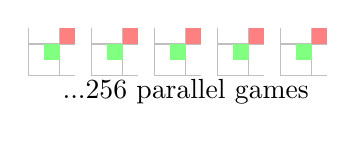
\begin{tikzpicture}[scale=0.4]
            \foreach \i in {0,1,2,3,4} {
                \draw[gray!50] (\i*2,0) grid (\i*2+1.5,1.5);
                \fill[green!50] (\i*2+0.5,0.5) rectangle (\i*2+1,1);
                \fill[red!50] (\i*2+1,1) rectangle (\i*2+1.5,1.5);
            }
            \node at (5,-0.5) {...256 parallel games};
        \end{tikzpicture}
    \end{center}
\end{frame}

%===============================================
% PRESENTER 5: Two-Snake Demonstration
%===============================================
\presentertitle{5}{Two-Snake Competition}

%-----------------------------------------------
% Slide: Two-Snake Environment
%-----------------------------------------------
\begin{frame}{Two-Snake Environment}
    \begin{columns}
        \begin{column}{0.5\textwidth}
            \textbf{Rules:}
            \begin{itemize}
                \item Two snakes compete
                \item Same food, same grid
                \item Collision = death
                \item First to 10 food wins
            \end{itemize}

            \vspace{0.3cm}
            \textbf{New Challenges:}
            \begin{itemize}
                \item Opponent prediction
                \item Food competition
                \item Defensive play
            \end{itemize}
        \end{column}

        \begin{column}{0.5\textwidth}
            \begin{center}
                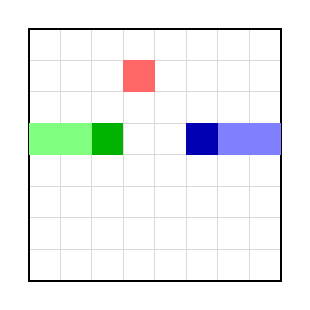
\begin{tikzpicture}[scale=0.4]
                    \draw[gray!30] (0,0) grid (8,8);
                    \draw[black, thick] (0,0) rectangle (8,8);

                    % Snake 1 (green)
                    \fill[green!50] (0,4) rectangle (1,5);
                    \fill[green!50] (1,4) rectangle (2,5);
                    \fill[green!70!black] (2,4) rectangle (3,5);

                    % Snake 2 (blue)
                    \fill[blue!50] (7,4) rectangle (8,5);
                    \fill[blue!50] (6,4) rectangle (7,5);
                    \fill[blue!70!black] (5,4) rectangle (6,5);

                    % Food
                    \fill[red!60] (3,6) rectangle (4,7);
                \end{tikzpicture}
            \end{center}
        \end{column}
    \end{columns}
\end{frame}

%-----------------------------------------------
% Slide: Naive Approach - Self-Play
%-----------------------------------------------
\begin{frame}{Naive Approach: Self-Play from Scratch}
    \textbf{Idea:} Both agents learn simultaneously against each other

    \vspace{0.5cm}
    \begin{columns}
        \begin{column}{0.5\textwidth}
            \textbf{How it works:}
            \begin{itemize}
                \item Both snakes start untrained
                \item Learn by playing each other
                \item Update both policies together
            \end{itemize}

            \vspace{0.3cm}
            \textbf{Problems:}
            \begin{itemize}
                \item Non-stationary environment
                \item Both agents are bad initially
                \item Unstable learning dynamics
            \end{itemize}
        \end{column}

        \begin{column}{0.5\textwidth}
            \begin{center}
                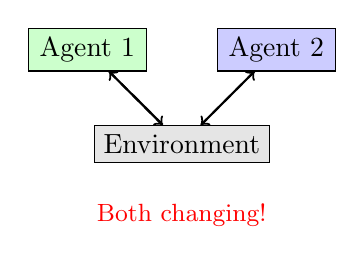
\begin{tikzpicture}[scale=0.6]
                    \node[draw, rectangle, fill=green!20, minimum width=1.5cm] (a1) at (0,0) {Agent 1};
                    \node[draw, rectangle, fill=blue!20, minimum width=1.5cm] (a2) at (4,0) {Agent 2};
                    \node[draw, rectangle, fill=gray!20, minimum width=2cm] (env) at (2,-2) {Environment};

                    \draw[->, thick] (a1) -- (env);
                    \draw[->, thick] (a2) -- (env);
                    \draw[->, thick, dashed] (env) -- (a1);
                    \draw[->, thick, dashed] (env) -- (a2);

                    \node[red] at (2,-3.5) {\small Both changing!};
                \end{tikzpicture}
            \end{center}
        \end{column}
    \end{columns}
\end{frame}

%-----------------------------------------------
% Slide: Self-Play Demo
%-----------------------------------------------
\begin{frame}{Self-Play Results}
    \begin{center}
        \textit{Both agents struggle to learn meaningful behavior}
    \end{center}
\end{frame}

%-----------------------------------------------
% Slide: Solution - Curriculum Learning
%-----------------------------------------------
\begin{frame}{Solution: Curriculum Learning}
    \textbf{Idea:} Train against progressively harder opponents

    \vspace{0.5cm}
    \begin{itemize}
        \item Start with simple, \textbf{fixed} opponents
        \item Agent learns basic skills first
        \item Gradually increase difficulty
        \item Only use self-play at the end
    \end{itemize}

    \vspace{0.5cm}
    \begin{center}
        \fbox{Stable opponents $\rightarrow$ stable learning}
    \end{center}
\end{frame}

%-----------------------------------------------
% Slide: Curriculum Learning
%-----------------------------------------------
\begin{frame}{Curriculum Learning Stages}
    \textbf{Train RL agent against progressively harder opponents:}

    \vspace{0.3cm}
    \begin{center}
        \begin{tabular}{clcc}
            \toprule
            \textbf{Stage} & \textbf{Opponent} & \textbf{Steps} & \textbf{Threshold} \\
            \midrule
            0 & Static & 0.5-1M & 95\% \\
            1 & Random & 0.5-1M & 95\% \\
            2 & Greedy & 3-6M & 35\% \\
            3 & Frozen (self) & 2-4M & 90\% \\
            4 & Co-evolution & 14M & --- \\
            \bottomrule
        \end{tabular}
    \end{center}

    \vspace{0.3cm}
    \begin{center}
        \fbox{Gradually increase opponent difficulty}
    \end{center}
\end{frame}

%-----------------------------------------------
% Slide: Two-Snake Demo
%-----------------------------------------------
\begin{frame}{Competitive Match Demo}
    \begin{center}
        \textit{Trained agents competing head-to-head}
    \end{center}
\end{frame}

%-----------------------------------------------
% Slide: Two-Snake Results
%-----------------------------------------------
\begin{frame}{Two-Snake Results}
    \textbf{Observed behaviors:}
    \begin{itemize}
        \item Aggressive food pursuit
        \item Defensive space control
        \item Opponent blocking strategies
    \end{itemize}

    \vspace{0.5cm}
    \textbf{Competition results (1000 games):}
    \begin{center}
        \begin{tabular}{lccc}
            \toprule
            \textbf{Method} & \textbf{256x256} & \textbf{128x128} & \textbf{Draw} \\
            \midrule
            DQN Direct & 0\% & 0\% & 100\% \\
            PPO Direct (2M) & 51\% & 31\% & 18\% \\
            PPO Direct (14M) & 33\% & 42\% & 26\% \\
            PPO Curriculum & 40\% & 38\% & 22\% \\
            \bottomrule
        \end{tabular}
    \end{center}
\end{frame}

%===============================================
% PRESENTER 6: Limitations & Future Development
%===============================================
\presentertitle{6}{Limitations \& Future}

%-----------------------------------------------
% Slide: Limitations - Sample Inefficiency
%-----------------------------------------------
\begin{frame}{Limitation: Sample Inefficiency}
    \begin{center}
        \includegraphics[width=0.5\textwidth]{"figures/sample inefficiency curves.png"}
    \end{center}

    \vspace{0.3cm}
    \begin{center}
        \fbox{Sample efficiency is the biggest bottleneck}
    \end{center}
\end{frame}

%-----------------------------------------------
% Slide: Training Results Grid
%-----------------------------------------------
\begin{frame}{Training Results Overview}
    \begin{center}
    \tiny
    \setlength{\tabcolsep}{1pt}
    \renewcommand{\arraystretch}{0.5}
    \begin{tabular}{cccc}
        \includegraphics[width=0.24\textwidth]{figures/training/dqn_basic_20251129_231638.png} &
        \includegraphics[width=0.24\textwidth]{figures/training/dqn_flood-fill_20251129_231638.png} &
        \includegraphics[width=0.24\textwidth]{figures/training/dqn_selective_20251129_231638.png} &
        \includegraphics[width=0.24\textwidth]{figures/training/dqn_enhanced_20251201_020448.png} \\
        \includegraphics[width=0.24\textwidth]{figures/training/double_dqn_basic_20251129_231638.png} &
        \includegraphics[width=0.24\textwidth]{figures/training/double_dqn_flood-fill_20251129_231638.png} &
        \includegraphics[width=0.24\textwidth]{figures/training/double_dqn_selective_20251129_231638.png} &
        \includegraphics[width=0.24\textwidth]{figures/training/double_dqn_enhanced_20251201_020450.png} \\
        \includegraphics[width=0.24\textwidth]{figures/training/dueling_dqn_basic_20251129_231638.png} &
        \includegraphics[width=0.24\textwidth]{figures/training/dueling_dqn_flood-fill_20251129_231638.png} &
        \includegraphics[width=0.24\textwidth]{figures/training/dueling_dqn_selective_20251129_231638.png} &
        \includegraphics[width=0.24\textwidth]{figures/training/dueling_dqn_enhanced_20251201_020452.png} \\
        \includegraphics[width=0.24\textwidth]{figures/training/noisy_dqn_basic_20251129_231638.png} &
        \includegraphics[width=0.24\textwidth]{figures/training/noisy_dqn_flood-fill_20251129_231638.png} &
        \includegraphics[width=0.24\textwidth]{figures/training/noisy_dqn_selective_20251130_165637.png} &
        \includegraphics[width=0.24\textwidth]{figures/training/noisy_dqn_enhanced_20251201_020454.png} \\
        \includegraphics[width=0.24\textwidth]{figures/training/per_dqn_basic_20251129_231638.png} &
        \includegraphics[width=0.24\textwidth]{figures/training/per_dqn_flood-fill_20251129_231638.png} &
        \includegraphics[width=0.24\textwidth]{figures/training/per_dqn_selective_20251130_204729.png} &
        \includegraphics[width=0.24\textwidth]{figures/training/per_dqn_enhanced_20251201_020456.png} \\
        \includegraphics[width=0.24\textwidth]{figures/training/ppo_basic_20251129_231638.png} &
        \includegraphics[width=0.24\textwidth]{figures/training/ppo_flood-fill_20251129_231638.png} &
        \includegraphics[width=0.24\textwidth]{figures/training/a2c_basic_20251129_231638.png} &
        \includegraphics[width=0.24\textwidth]{figures/training/a2c_flood-fill_20251129_231638.png} \\
    \end{tabular}
    \end{center}
\end{frame}

%-----------------------------------------------
% Slide: Limitations - Unreliability
%-----------------------------------------------
\begin{frame}{Limitation: Unreliability}
    \textbf{Sensitive to initial conditions:} Same algorithm, different random seed

    \vspace{0.3cm}
    \begin{center}
        \includegraphics[width=0.7\textwidth]{"figures/sample algorithm different seeds.png"}
    \end{center}

    \vspace{0.3cm}
    \begin{center}
        \textit{Results vary dramatically with different seeds}
    \end{center}
\end{frame}

%-----------------------------------------------
% Slide: Other Limitations
%-----------------------------------------------
\begin{frame}{Other Limitations}
    \begin{itemize}
        \item \textbf{Reward Engineering} -- Designing good reward functions is difficult
        \vspace{0.3cm}
        \item \textbf{Sim-to-Real Gap} -- Policies trained in simulation may not transfer
        \vspace{0.3cm}
        \item \textbf{Safety} -- Exploration can be dangerous in real world
        \vspace{0.3cm}
        \item \textbf{Hyperparameter Sensitivity} -- Small changes can break training
    \end{itemize}
\end{frame}

%-----------------------------------------------
% Slide: Future Development in RL
%-----------------------------------------------
\begin{frame}{Future Development in RL}
    \begin{itemize}
        \item \textbf{Bayesian RL} -- Reason about uncertainty
        \item \textbf{Distributional RL} -- Learn full return distribution
        \item \textbf{Imitation Learning} -- Learn from expert demonstrations
        \item \textbf{RLHF} -- Align with human preferences
    \end{itemize}
\end{frame}

%-----------------------------------------------
% Slide: Real-World Applications
%-----------------------------------------------
\begin{frame}{Real-World Applications}
    \begin{itemize}
        \item \textbf{Games \& Simulation} -- AlphaGo, AlphaZero, OpenAI Five (Dota 2)
        \vspace{0.3cm}
        \item \textbf{Robotics} -- Locomotion, Navigation
        \vspace{0.3cm}
        \item \textbf{Real-World Systems} -- Autonomous vehicles
        \vspace{0.3cm}
        \item \textbf{Language Models} -- RLHF for LLMs
    \end{itemize}
\end{frame}

%-----------------------------------------------
% Slide: Key Takeaway
%-----------------------------------------------
\begin{frame}{Key Takeaway}
    \begin{center}
        \vspace{1.5cm}
        {\Large \textbf{RL is a powerful tool}}

        \vspace{0.5cm}
        {\Large \textbf{if you know how to engineer it}}

        \vspace{1.5cm}
        \textbf{Techniques:} Feature engineering, Algorithm choice, Hyperparameters, Curriculum learning, GPU acceleration
    \end{center}
\end{frame}

%-----------------------------------------------
% Slide: References
%-----------------------------------------------
\begin{frame}{References}
    \begin{itemize}
        \item Sutton, R. S., \& Barto, A. G. (2018). \textit{Reinforcement Learning: An Introduction} (2nd ed.). MIT Press.
        \item Mnih, V., et al. (2015). Human-level control through deep reinforcement learning. Nature.
        \item Schulman, J., et al. (2017). Proximal Policy Optimization Algorithms.
        \item OpenAI. \textit{Spinning Up in Deep RL}. https://spinningup.openai.com/
        \item Irpan, A. (2018). \textit{Deep Reinforcement Learning Doesn't Work Yet}. https://www.alexirpan.com/2018/02/14/rl-hard.html
    \end{itemize}
\end{frame}

%-----------------------------------------------
% Slide: Q&A
%-----------------------------------------------
\begin{frame}{Questions?}
    \begin{center}
        \vspace{2cm}
        {\Huge \textbf{Q\&A}}

        \vspace{1cm}
        \textit{Thank you for your attention!}
        \vspace{2cm}
    \end{center}
\end{frame}

%-----------------------------------------------
% Blank Slide
%-----------------------------------------------
\begin{frame}
\end{frame}

\end{document}
